
\begin{TP}[Figure de Kolam]

\begin{minipage}[t]{0.48\linewidth}
Dans l'État du Tamil Nadu, dans le sud-est de l'Inde, les mères enseignent à leurs filles l'art de dessiner avec de la poudre de riz des figures de Kolam qui décorent le seuil des habitations.
 \end{minipage} \hfill%
 \begin{minipage}[t]{0.48\linewidth}
 \begin{enumerate}
  \item Sur une feuille blanche, reproduisez la figure $A$ ;
  \item Complétez la figure $A$ afin d'obtenir la figure $B$ en effectuant des rotations. Trouvez le centre des rotations ;
  \item Complétez la figure pour obtenir la figure C. 
  \end{enumerate}
  \end{minipage} \\
  
\begin{minipage}[t]{0.32\linewidth}
 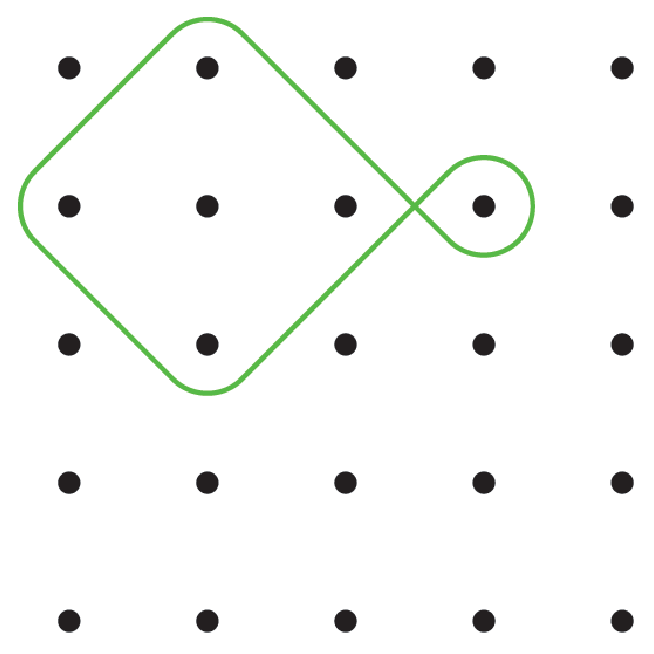
\includegraphics[width=3.6cm]{Kolam1}
 \end{minipage} \hfill%
 \begin{minipage}[t]{0.32\linewidth}
  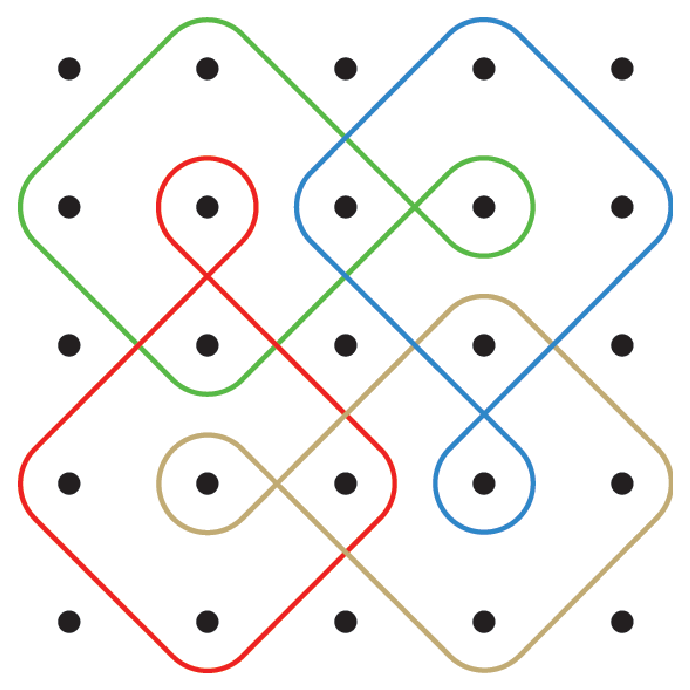
\includegraphics[width=3.6cm]{Kolam2}
  \end{minipage} \hfill%
  \begin{minipage}[t]{0.32\linewidth}
   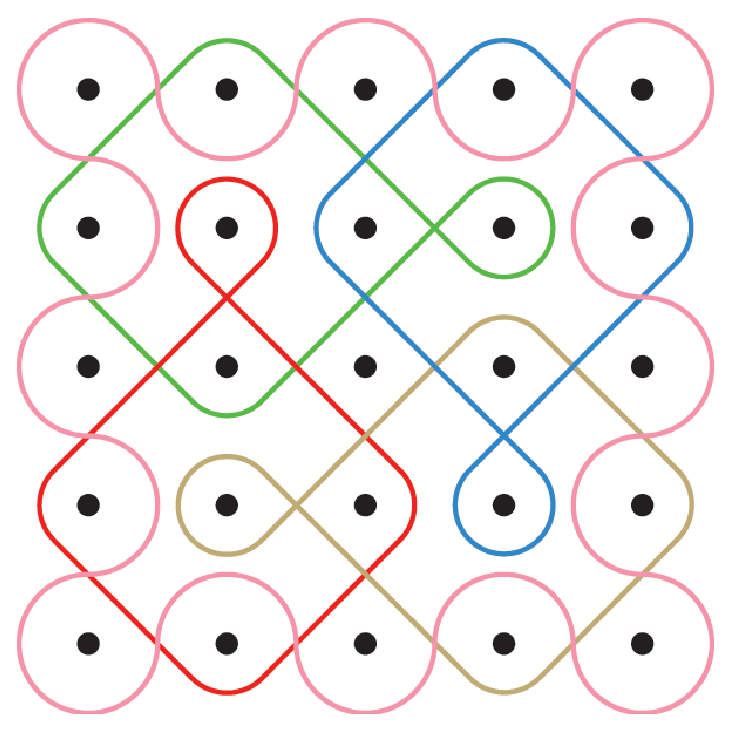
\includegraphics[width=3.6cm]{Kolam3}
   \end{minipage} \\

\end{TP}

